\section{Runtime Halo Finder}
\label{sec:halo}

%Spherical overdensities, search algorithm, 
%provided halo information, halo bias, comparison to PS and ST.
%{\bf (Ilian, You can lead the way here...)}

We have implemented a halo finding procedure, which we have developed 
based on the spherical overdensity (SO) approach \citep{1994MNRAS.271..676L}.
In the interest of speed and efficiency the halo catalogues are constructed 
on-the-fly at a pre-determined list of redshifts. The halo finding is 
massively-parallel and threaded based on the main {\small CUBEP3M} data structures 
discussed in section \ref{sec:structure}. The code first builds the 
fine-mesh density for each sub-domain using CIC or NGP interpolation. It then 
proceeds to search for all local density maxima above a certain
threshold (typically set to a factor of 100 above mean density) within the local tile. 
It then uses parabolic interpolation on the density field to determine more precisely
the location of the maximum within the densest cell, and records the peak 
position and value. %The halo centre determined this way agrees closely with 
%the centre-of-mass of the halo particles discussed below.  

Once the list of peak positions is generated, they are sorted from the highest 
to the lowest density value. Then each of the halo candidates is inspected 
independently, starting with the highest peak. The grid mass is accumulated 
in spherical shells of fine grid cells surrounding the maximum, until the 
mean density within the halo drops below a pre-defined overdensity cutoff 
(usually set to 178 in units of the mean, in accordance with the top-hat 
collapse model). As we accumulate the mass, we remove it from the mesh, so that no 
mass element is double-counted. This method is thus inappropriate for finding 
sub-haloes since within this framework, those are naturally incorporated in their 
host haloes. Because the haloes are found on a discrete grid, it is 
possible, especially for those with lower mass, to overshoot the target overdensity.
To minimize this efect, we correct the halo mass and radius with an analytical density profile. 
We use the Truncated Isothermal Sphere (TIS) 
profile \citep{1999MNRAS.307..203S,2001MNRAS.325..468I} for overdensities below 
$\sim130$, and a simple $1/r^2$ law for lower overdensities {\bf (lower or higher?)}. 
These yield a similar outer slope to the Navarro, Frenk and White 
\citep[NFW][]{1997ApJ...490..493N} profile, but extends to lower overdensities
and matches well the virialization shock position given by the Bertschinger 
self-similar collapse solution \citep{1985ApJS...58...39B}.

Once the correct halo mass, radius and position are determined, we find all 
particles that are within the halo radius. Their positions and velocities are
used to calculate the halo centre-of-mass, bulk velocity, internal velocity 
dispersion and the three angular momentum components, all of which are then 
included in the final halo catalogues. We also calculate the total mass of
all particles within the halo radius, also listed in the halo data. This mass
is very close, but  typically slightly lower, than the halo mass calculated 
based on the gridded density field. The  centre-of-mass found this way closely follows 
that found from the peak location, which is based on the gridded mass distribution. 

%Compared to Tinker
%44% low for 50 particles
%22% low for 400 particles
%12% low for 1000 particles

\begin{figure}%[ht]
%  \vskip -0.5cm 
  \begin{center}
    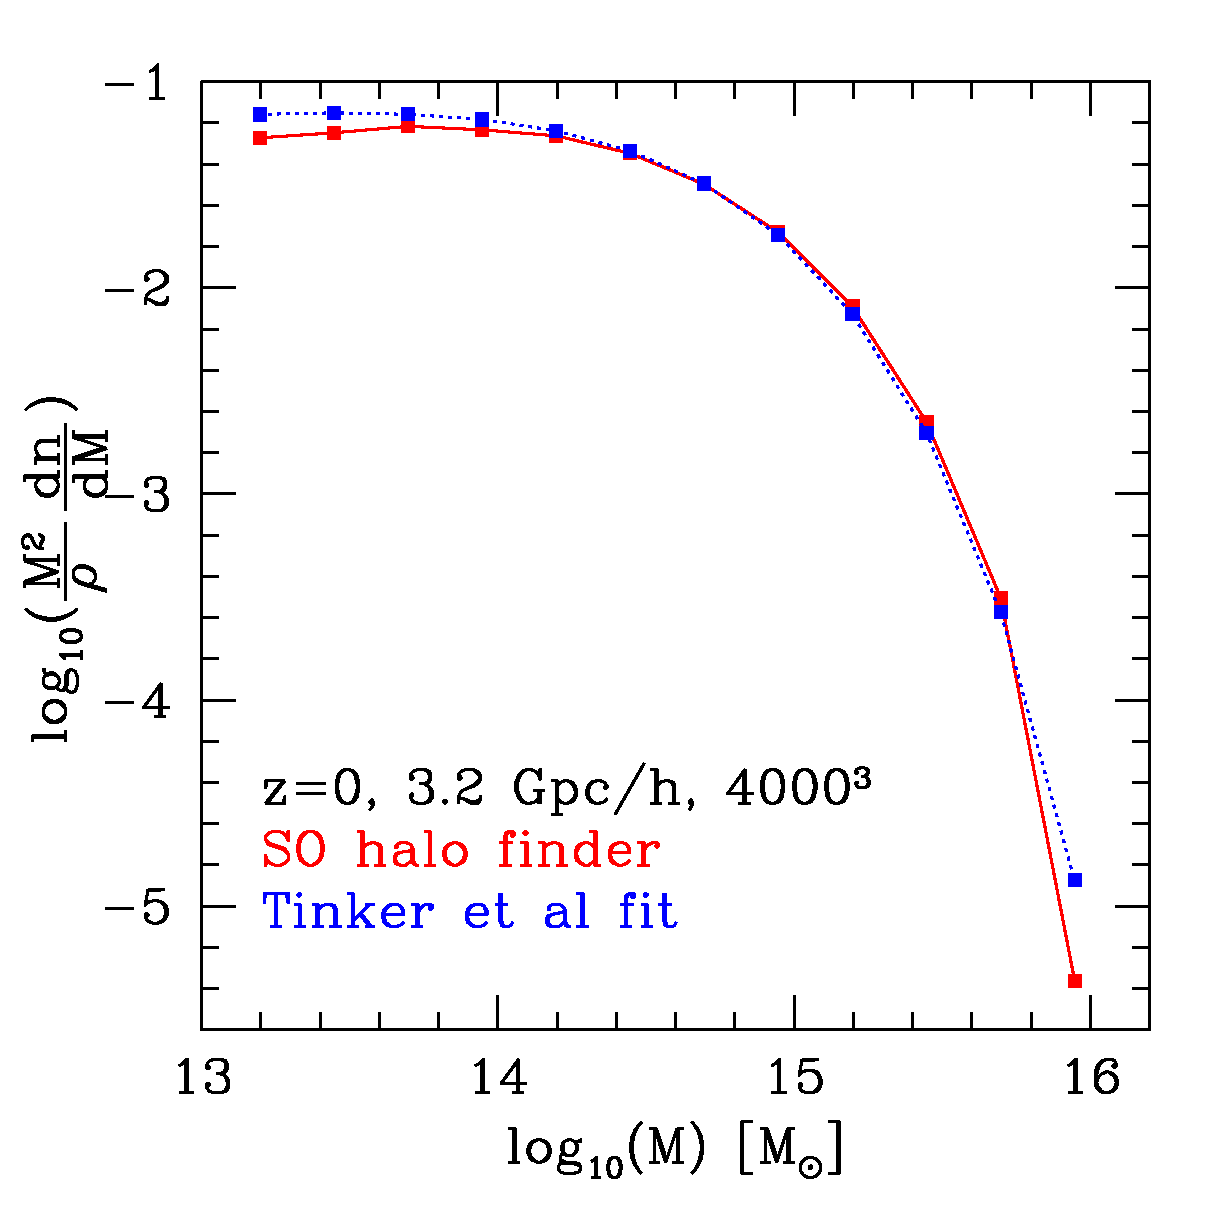
\includegraphics[width=3.2in]{graphs/mf_z0_Tinker.eps}
  \end{center}
  \caption{Simulated halo multiplicity function, 
    $\frac{M^2}{\bar{\rho}}\frac{dn}{dM}$, based on a
    RANGER4000 simulation with $3.2\,h^{-1} \mbox{Gpc}$ box and $4000^3$ 
    particles (solid, red in the online version). For reference we also show a widely-used 
    precise fit by \citet{2008ApJ...688..709T} (blue, dashed). 
    \label{mf}}
\end{figure}

A sample halo mass function produced  from a RANGER4000 simulation at $z=0$ is shown in Fig. \ref{mf}. We compare our result to the 
precise fit presented recently by \citet{2008ApJ...688..709T}. Unlike most
other widely-used fits like the one by \citet{2002MNRAS.329...61S}, which are based on friends-of-friends (FOF)
halo finders, this one is based on the
SO search algorithm, whose masses are systematically different 
from the FOF masses \citep[e.g.][]{2007MNRAS.374....2R,2008ApJ...688..709T}, 
making this fit a better base for comparison here. Results show excellent
agreement, within $\sim10$ per cent for all haloes with masses corresponding to
1000 particles or more. Lower-mass haloes are somewhat under-counted compared
to the \citet{2008ApJ...688..709T} fit, by $\sim20$ per cent for 400 particles and 
by $\sim40$ per cent for 50 particles. This is due to the grid-based nature of our
SO halo finder, which misses some of the low-mass haloes. It was shown, however, that using more sophisticated
halo finders (available only through post-processing calculations due to their heavier memory
footprint) it is possible to recover the expected mass function.

%A second test of the accuracy of the halo finder algorithm is to extract the halo power spectrum $P_{h}(k)$ and compare the halo bias
%with theoretical predictions. The halo bias is defined as $b(k) = \sqrt{P(k)/P_{h}(k)}$ and is shown in Fig. \ref{fig:halo}.
%The results are organized in four mass bins, where the lowest mass consists of 20-200 particles, the second bin 
%contains 200-2000 particles and so on. Comparisons with the linear predictions of \citet{2001MNRAS.323....1S} shows
%results consistent the known flaws of the model, namely that low-mass bias is over-predicted and high-mass bias is under-predicted \citep{2010ApJ...724..878T}.
%
%\begin{figure}%[ht]
%  \vskip -0.5cm 
%  \begin{center}
%    \includegraphics[width=3.2in]{graphs/bias.eps}
%  \end{center}
%  \caption{Halo bias, measured at $z=0$ from a RANGER4000 simulation with a side length of $3.2 h^{-1}$Gpc.
%  Bottom to top curves correspond to haloes of different masses, from light to massive. The four bins are decades
%  of halo masses; the first contains haloes made of 20-200 particles, the second of 200-2000 and so on.
%  The dashed lines are linear predictions from \protect \citet{2001MNRAS.323....1S}.
%    \label{fig:halo}}
%\end{figure}


%{\bf Show some examples and comparisions to analytical fits and other halo finders.}
